\documentclass[t, 9pt]{beamer}
\mode<presentation>
{
  \usetheme{Warsaw}
  %\usefonttheme{serif}
}
%\mode<presentation>
%{
%\usetheme{Warsaw}
%}
%\usefonttheme{structuresmallcapsserif}

%----------------------------------------
%            PACKAGES
%----------------------------------------

%--FIGURES
\usepackage{graphicx}
\usepackage{subfigure}

%--FONT
%upright mu - \textmu
%\usepackage{textcomp} 
\usepackage{amsmath}
\usepackage{amssymb}
\usepackage[bold]{hhtensor}
\usepackage{array}
%-----TIKZ
\usepackage{circuitikz}
\usepackage{ifthen}
\usepackage{tikz}
\usepackage{pgf}
\usepackage{pgffor}
\usepgfmodule{shapes}
\usepgfmodule{plot}
\usetikzlibrary{decorations}
\usetikzlibrary{arrows}
\usetikzlibrary{snakes}
\usetikzlibrary{arrows,positioning} 
\tikzset{
    %Define standard arrow tip
    >=stealth',
    %Define style for boxes
    punkt/.style={
           rectangle,
           rounded corners,
           draw=black, very thick,
           text width=6.5em,
           minimum height=2em,
           text centered},
    % Define arrow style
    pil/.style={
           ->,
           thick,
           shorten <=2pt,
           shorten >=2pt,}
}

\usepackage{xcolor}
\def\setcolormodel{cmyk}

%--HYPERLINKS
%\hypersetup{colorlinks=true,       % false: boxed links; true: colored links
%	linkcolor=OliveGreen,          % color of internal links
%	citecolor=BrickRed,        % color of links to bibliography
%	urlcolor=Blue,
%	bookmarksnumbered=true,
%	pdffitwindow=true, 
%	bookmarks=true}         % show
\usepackage{url}

%--GRAPHICS PATH
\graphicspath{{~/Dropbox/github/TOM/figures/}}



%--Title slide configuration
% !TEX root = F429_1s1014.tex




%--BEGIN DOCUMENT HERE!
\begin{document}    

%\begin{frame}[allowframebreaks]{Power Dissipation in RLC circuits}
%As current and voltage are time-dependent functions, we can define an instantaneous power dissipated in a given circuit component with a voltage drop $v(t)$ as
%\begin{equation}
%  P(t)=v(t)i(t),
%\end{equation}
%where i(t) is the current flowing through the circuit component. Writing $v(t)=v_0\cos(\omega t)$, $i(t)=v_0\cos(\omega t+\phi)$ we obtain,
%\begin{equation}
%  P(t)=\frac{1}{2}\left(v_0 i_0\cos(\phi)+\cos(2\omega t+\phi)\right),
%\end{equation}
%The average power (over one period, $T=2\pi/\omega$) can be obtained as,
%\begin{equation}
%  \bar{P}\equiv\frac{1}{T}\int_0^{T}P(t)=\frac{1}{2}v_0 i_0\cos(\phi),
%\end{equation}
%Two aspects must be noticed from Eq. above
%\begin{itemize}
%  \item 
%\end{itemize}
%\pause
%	\begin{columns}
%		\begin{column}{0.5\textwidth}
%
%		In figure we show the time dependence of the instantaneous power (yellow curve) together with a unit voltage ($v_0=1$, blue curve) and a unit current ($i_0=1$, red curve) and $\phi=45^{\circ}$. The green curve shows the average power $\bar{P}$. 
%					\end{column}
%		\begin{column}{0.5\textwidth}
%			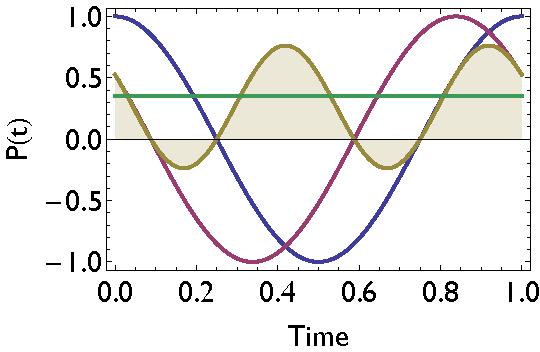
\includegraphics[width=.8\textwidth]{/Users/gsw/github/F429/potencia_instantanea_phi45.pdf}
%
%		\end{column}
%	\end{columns}
%From Ohm's law we now that current can be easily measured from the voltage drop across the circuit's resistor $i(t)=\frac{1}{R}v_R(t)$
%	\begin{columns}
%		\begin{column}{0.5\textwidth}
%			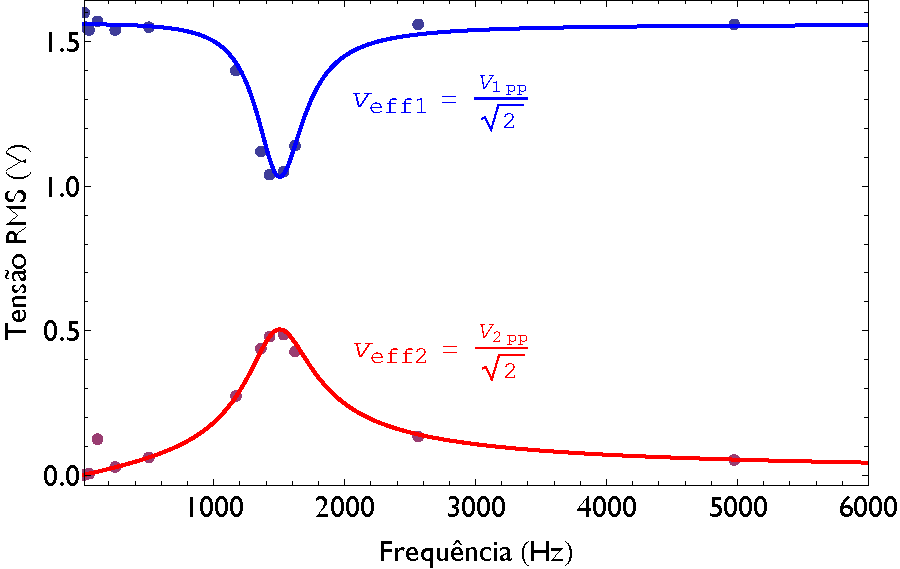
\includegraphics[width=\textwidth]{/Users/gsw/github/F429/v1_v2_eff_rlc.pdf}
%		\end{column}
%		\begin{column}{0.5\textwidth}
%			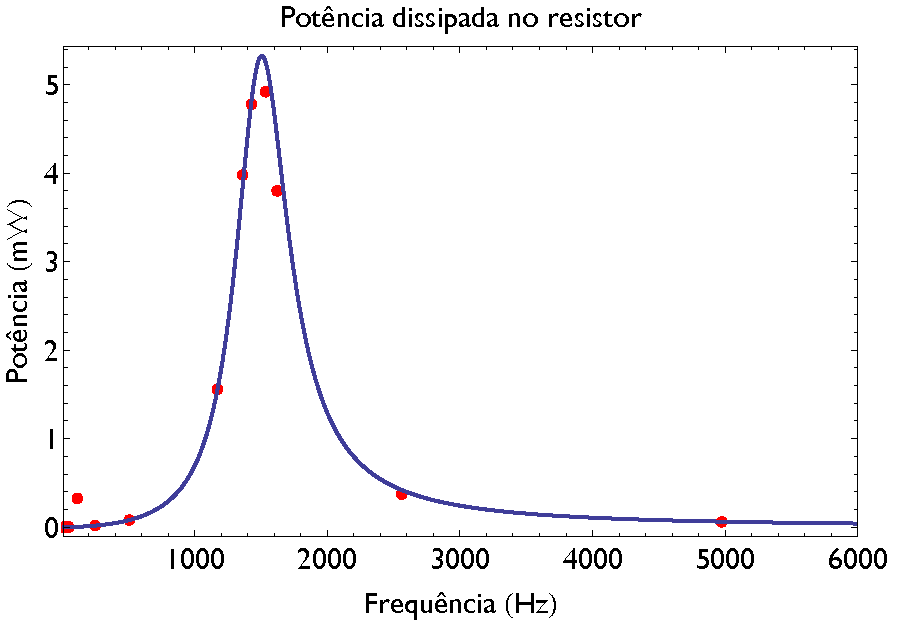
\includegraphics[width=\textwidth]{/Users/gsw/github/F429/pdiss_rlc.pdf}
%		\end{column}
%	\end{columns}
%
%
%\end{frame}
%
%\begin{frame}
%
%From Ohm's law we now that current can be easily measured from the voltage drop across the circuit's resistor $i(t)=\frac{1}{R}v_R(t)$
%\pause
%\begin{columns}
%	\begin{column}{0.5\textwidth}
%		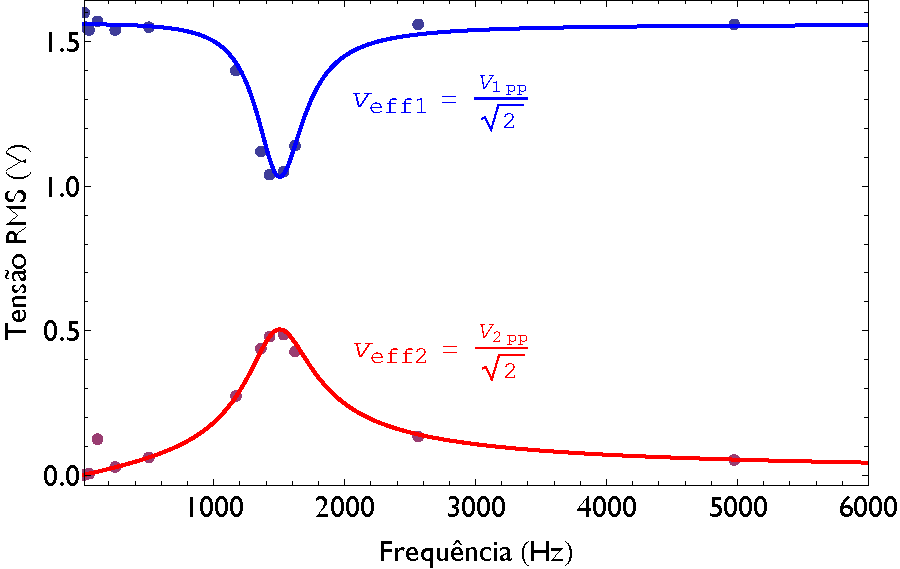
\includegraphics[width=\textwidth]{/Users/gsw/github/F429/v1_v2_eff_rlc.pdf}
%	\end{column}
%	\begin{column}{0.5\textwidth}
%		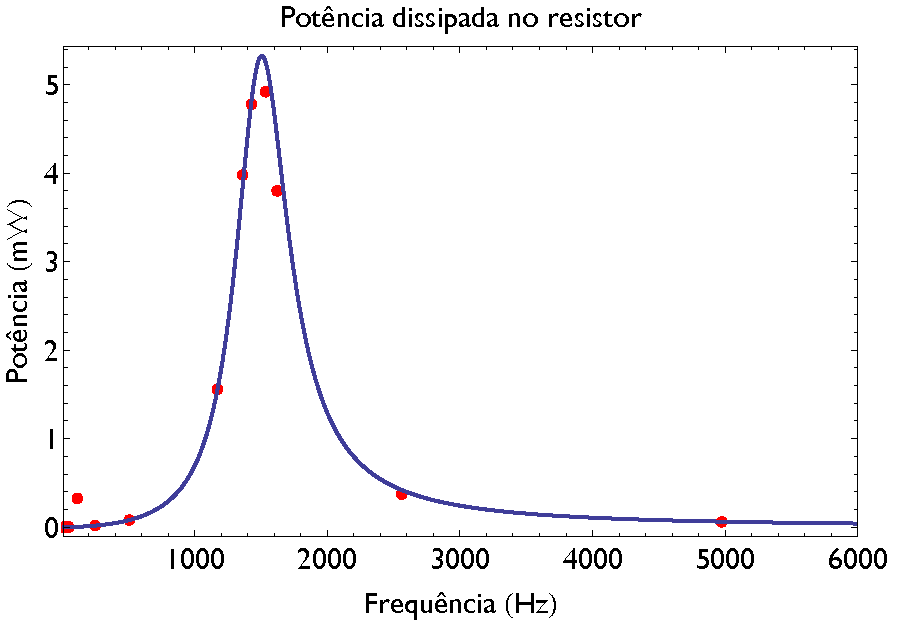
\includegraphics[width=\textwidth]{/Users/gsw/github/F429/pdiss_rlc.pdf}
%	\end{column}
%\end{columns}
%\begin{align*}
%    \only<1-1>{E=mc^1}
%    \only<2-2>{E=mc^2}
%    \only<3-3>{E=mc^3}
%\end{align*}
%
%\end{frame}

% Typing shortcuts
%---------------------------------------------------------------------
%            SHORTCUTS USED IN THE TEXT
%---------------------------------------------------------------------
% CUSTOM SHORTCUTS
\newcommand{\neff}{n_\text{eff}}
\newcommand{\ml}{Matlab\textsuperscript{\textregistered} }
\newcommand{\cm}{Comsol\textsuperscript{\textregistered} }
\newcommand{\sinn}{Si$_3$N$_4$\text{ }}
\newcommand{\sio}{SiO$_2$\text{ }}
%
%\newcommand*{\eps0}{ \epsilon_0 }
%\newcommand{\mu0}{\mu$_0$}

%------------------------------------------
%vector calculus
\newcommand{\divg}[1]{\nabla \cdot \vec{#1}}
\newcommand{\rot}[1]{\nabla \times \vec{#1}}

%------------------------------------------
%time derivatives
\newcommand{\dpt}[1]{\frac{\partial \vec{#1}}{\partial t}}
\newcommand{\dt}[1]{\frac{d \vec{#1}}{d t}}

%------------------------------------------
%			TWO PORT NETWORK
%------------------------------------------
\newcommand{\tpn}[2]{
	\begin{circuitikz}[scale=1]
		\node (Xi) at (0.7,0.7) {$V_1$};
		\node (Xf) at (3.7,0.7) {$V_2$};
		\draw [semithick,->] (Xi) -- (0.1,0.1);
		\draw [semithick,->] (Xf) -- (3.1,0.1);
		\draw
			to [generic, o-o, l_=$#1$] ++(2,0)
			(2,0) to [short,o-o] ++(1,0)
			(2,0) to [generic, o-o, l=$#2$] ++(0,-2)
			node[ground] {}
			;
	\end{circuitikz}
}

\newcommand{\tpn}[2]{
	\begin{circuitikz}[scale=1]
		\node (Xi) at (0.7,0.7) {$V_1$};
		\node (Xf) at (3.7,0.7) {$V_2$};
		\draw [semithick,->] (Xi) -- (0.1,0.1);
		\draw [semithick,->] (Xf) -- (3.1,0.1);
		\draw
			to [generic, o-o, l_=$#1$] ++(2,0)
			(2,0) to [short,o-o] ++(1,0)
			(2,0) to [generic, o-o, l=$#2$] ++(0,-2)
			node[ground] {}
			;
	\end{circuitikz}
}	
%------------------------------------------
%			PHASOR DIAGRAM
%------------------------------------------
\newcommand{\Gitter}[4]{
    \draw[very thin,color=gray] (#1,#3) grid (#2,#4);
}
\newcommand{\Koordinatenkreuz}[6]{
    \draw[->, >=latex, color=green!50!black] (#1,0) -- (#2,0) node[right] {#5};
    \draw[->, >=latex, color=green!50!black] (0,#3) -- (0,#4) node[left] {#6};
}
\newcommand{\KoordinatenkreuzOhneLabelsVerschobenKeinPfeil}[5]{
    \draw[-] (#1,0) -- (#2,0);
    \draw[-] (#5,#3) -- (#5,#4);

}
\newcommand{\ZeigerdiagrammText}[4]{
\begin{tikzpicture}[scale=.72, samples=100, >=latex]

    \def\Alpha{#1}
    \def\Phase{#2}
    \def\AmplitudeSpannung{#3}
    \def\AmplitudeStrom{#4}
    \def\SpannungsWert{{\AmplitudeSpannung*sin(\Alpha)}}
    \def\StromWert{{\AmplitudeStrom*sin(\Alpha+\Phase)}}
    %%%%%%%%%%%%%%%%%%%%%%%%%%%%%%%%%%%%%%%%%%%%%%%%%%%%%%%%%%
    \def\FarbeSpannung{blue!90!white}
    \def\FarbeStrom{red!90!white}
    \def\FarbeWinkelZeichnung{green}
    %%%%%%%%%%%%%%%%%%%%%%%%%%%%%%%%%%%%%%%%%%%%%%%%%%%%%%%%%%
    \def\Beta{\Alpha+\Phase}
    \def\AlphaRad{\Alpha*3.141592654/180}
    \def\PhaseRad{\Phase*3.141592654/180}
    %%%%%%%%%%%%%%%%%%%%%%%%%%%%%%%%%%%%%%%%%%%%%%%%%%%%%%%%%%
    \Gitter{-.1}{7.1}{-3.1}{3.1}
    \Koordinatenkreuz{-.2}{7.3}{-3.2}{3.3}{$\omega t$}{}
    \draw (1.570795,0) node[below]{$\frac{\pi}{2}$};
    \draw (3.14159,0) node[below]{${\pi}$};
    \draw (4.71238898,0) node[below]{$\frac{3\pi}{2}$};
    \draw (6.283185307,0) node[below]{${2\pi}$};
    \draw (-4,0) circle (3cm);
    \KoordinatenkreuzOhneLabelsVerschobenKeinPfeil{-7.2}{-.8}{-3.6}{3.6}{-4}
    %%%%%%%%%%%%%%%%%%%%%%%%%%%%%%%%%%%%%%%%%%%%%%%%%%%%%%%%%%

    % voltage
    \draw[color=\FarbeSpannung, very thick] plot[id=voltage, domain=0:7] function{\AmplitudeSpannung*sin(x)} node[right] {$U(t)$};
    % voltage circle
    \draw[color=\FarbeSpannung, loosely dashed] (-4,0) circle (\AmplitudeSpannung cm);
    % angle
    \draw[color=\FarbeWinkelZeichnung!50!black, thick] (\AlphaRad, \SpannungsWert)--(\AlphaRad,\StromWert) node[below=18pt] {$\alpha$};
    % angle in the circle
    \filldraw[fill=\FarbeWinkelZeichnung!20,draw=\FarbeWinkelZeichnung!50!black] (-4,0) -- (-3,0) arc (0:\Alpha:1) -- cycle node[right] {$\alpha$};
    % voltage pointer
    \draw[<-,color=\FarbeSpannung, very thick] (\Alpha:\AmplitudeSpannung)++(-4,0) --(-4,0);
    \draw[color=\FarbeSpannung,  dashed] (\Alpha:\AmplitudeSpannung)++(-4,0) -- (\AlphaRad,\SpannungsWert);
    % current
    \draw[color=\FarbeStrom, very thick] plot[id=current, domain=0:7] function{\AmplitudeStrom*sin(x+\PhaseRad)} node[right] {$I(t)$};		
    % current circle
    \draw[color=\FarbeStrom, loosely dashed]    (-4,0) circle (\AmplitudeStrom cm);
    % current pointer
    \draw[<-,color=\FarbeStrom, very thick] (\Beta:\AmplitudeStrom)++(-4,0) --(-4,0);
    \draw[color=\FarbeStrom,  dashed](\Beta:\AmplitudeStrom)++(-4,0) -- (\AlphaRad,\StromWert);
    % phase difference
    \ifthenelse{\Phase<0}{
        \draw[snake=brace] (pi/2 ,3.3)--(pi/2-\PhaseRad ,3.3) node[above=7pt, left=10pt] {$\phi$};
    }
    {
        \draw[snake=brace] (pi/2-\PhaseRad ,3.3)--(pi/2 ,3.3) node[above=7pt, left=10pt] {$\phi$};
    }
    % angular velocity \omega
    \draw[->, xshift=-4cm]  (120:2.4cm) arc (120:170:2) node[below] {$\omega$};
\end{tikzpicture}
}
% Shortcut fot tables and figures.
\def\figurename{Fig.}
\def\tablename{Tab.}


%----------------------------------------
%-- SLIDES BEGIN HERE!!
%----------------------------------------

% Title slide
\begin{frame}
  \titlepage
\end{frame}

\AtBeginSection[]
{
\begin{frame}<beamer>{Table of Contents}
\tableofcontents[currentsection,currentsubsection, 
    hideothersubsections, 
    sectionstyle=show/shaded,
]
\end{frame}
}

% Maxwell Equations
\section{Two-port circuits}
\subsection{Generic two-port circuits}
\begin{frame}{Generic two-port circuits}
During the next experiments we will explore a few configurations of two-port circuits. The typical setup will be similar to Fig. \ref{fig:Generic_two_port} below.
\begin{figure}[hbt]
	\begin{circuitikz}
		\draw
			(0,0) node[ground] {}
			to [sinusoidal voltage source, o-o, l=$\epsilon(t)$] ++(0,2)
			to [generic, o-o, l=$Z_g$] ++(2,0)
			to [generic, o-o, l=$Z_1$] ++(2,0)
			(4,2) to [short,o-o,l_=a] ++(1,0)
			(4,2) to [generic, o-o, l=$Z_2$] ++(0,-2)
			node[ground] {}
			;
		%Description of subparts
		\draw [decorate,decoration={brace,amplitude=8pt},
					xshift=0pt, yshift=0pt]
					(2,-1) -- (-0.5,-1)
					node[black,midway,yshift=-20pt]
						{AC generator};
		\draw [decorate,decoration={brace,amplitude=8pt},
					xshift=0pt, yshift=0pt]
					(5,-1) -- (2.1,-1)
					node[black,right,yshift=-20pt]
						{Two-port circuit};	
	\end{circuitikz}
  \caption{\tiny{Generic two-port circuit setup. $Z_g$ represents the internal impedance of the AC generators, $Z_1,Z_2$ are any generic linear circuit components. The arrows $V_1$ and $V_2$ indicate where we connect  oscilloscope channels to the circuit. }}
  \label{fig:Generic_two_port}
\end{figure}

\end{frame}

\begin{frame}{Resistive voltage divider}
The simplest example of a two-port circuit is the voltage divider 			you learned in F328/F329 \cite{Walker:2008aa}. You obtain it by 			simple replacing $Z_{1,2}$ from Fig. \ref{fig:Generic_two_port} with two resistors.
	\begin{columns}
		\begin{column}{0.5\textwidth}
			\tpn{R_1}{R_2}
				\end{column}
		\begin{column}{0.5\textwidth}
		From KCL (Kirchhoff Circuit's Law):
			\begin{eqnarray}
			\Rightarrow v_1(t)=R_1 i(t)+ R_2 i(t)\\
			\Rightarrow i(t)=\frac{v_1(t)}{R_1+R_2}
			\label{eq:voltagediv_i}
  			\end{eqnarray}
		The voltage drop measured in channel 2 is given by
		\begin{equation}
  			v_2(t)=R_2 i(t)=\frac{R_2}{R_1+R_2}v_1(t)
  			\label{eq:voltagediv_v2}
		\end{equation}
		
		\end{column}
	\end{columns}
\end{frame}

\begin{frame}{Resistive voltage divider}
Based on Eq. \ref{eq:voltagediv_v2}, it is obvious now why such a circuit is called the voltage divider; the voltage measured on the \textbf{output port} of the circuit ($v_2$) is a fraction of the \textbf{input port} voltage ($v_1$).
	\begin{columns}
		\begin{column}{0.4\textwidth}
			\tpn{R_1}{R_2}
		\end{column}
		\begin{column}{0.6\textwidth}
		Using Eqs. \ref{eq:voltagediv_i} and \ref{eq:voltagediv_v2} one can now define the \textbf{frequency response} of the resistive voltage divider. For a given sinusoidal input, $v_1(t)=V_1\sin(\omega t)$, the output voltage will be given by 
\begin{equation}
  v_2(t)=\frac{R_2}{R_1+R_2}V_1\sin(\omega t)
  \label{eq:voltagediv_v2_freq}
\end{equation}
From Eq. \ref{eq:voltagediv_v2_freq} it is clear that the output voltage is \textbf{in-phase} with the input voltage but with a different amplitude.

		\end{column}
	\end{columns}
\end{frame}

\begin{frame}{Resistive voltage divider}
One can then define an output voltage $v_2(t)=V_2\sin(\omega t)$, where the amplitude $V_2=\frac{R_2}{R_1+R_2}V_1$. We now define a important quantity:
\begin{definition}
The response function of the two-port circuit network $H(\omega)$ is input-output relation $H(\omega)\equiv\frac{V_2(\omega)}{V_1(\omega)}$.
\end{definition}
Note however that although we included an explicit frequency dependence on the $H(\omega)$, in the trivial case of the resistive voltage divider $H=R_2/(R_1+R_2)$ does not depend on frequency. That simply reflects the fact that the voltage drop in a resistor is proportional to the current flowing through it.\\ In the laboratory it means that regardless of the AC generator frequency, the ratio of the voltage amplitudes measured in channels 1,2 will always be given by  $R_2/(R_1+R_2)$.
%		\begin{columns}
%			\begin{column}{0.5\textwidth}
%				\tpn{R_1}{R_2}
%			\end{column}
%			\begin{column}{0.5\textwidth}
%			
%			\end{column}
%		\end{columns}
\end{frame}

\begin{frame}{Resistive voltage divider: Numerical example}

\end{frame}

\subsection{RC voltage divider - Filters}

\begin{frame}{RC voltage divider}
We can try to apply the same principles used in the resistive voltage divider to a slightly more complex one, involving both a resistor and a capacitor. You shold also have learned about this circuit in F328/F329 \cite{Walker:2008aa}. You obtain it by 			simple replacing $Z_{1,2}$ from Fig. \ref{fig:Generic_two_port} with a capacitor and a resistor.
	\begin{columns}
		\begin{column}{0.5\textwidth}
			\tpn{R}{C}
			\tpn{C}{R}
				\end{column}
		\begin{column}{0.5\textwidth}
		From KCL (Kirchhoff Circuit's Law):
			\begin{equation}
			\Rightarrow v_1(t)=R i(t)+  q(t)/C
			\label{eq:rc_1}
  			\end{equation}
  			In contrast with the resistive divider (Eq. \ref{eq:voltagediv_i}), Eq. \ref{eq:rc_1} is an ordinary differential equation (ODE). Note that either circuit shown in the left follows the same equation. The difference is the voltage drop measured in channel 2 which will be given by
		\begin{eqnarray}
		     v_2(t)=q(t)/C\\
		     v_2(t)=R i(t)
  			\label{eq:rc_v2}
		\end{eqnarray}
		
		\end{column}
	\end{columns}
\end{frame}

\begin{frame}{RC voltage divider}
In order for to Eqs. \ref{eq:rc_v2} to be useful, one must solve the ODE \ref{eq:rc_1}. It is a inhomogeneous ODE where the dependent variable is the charge $q(t)$. We can decompose its solution in two parts, $q(t)=q_h(t)+q_p(t)$, where $q_h(t)=q_0 \exp(-t/\tau)$ is the solution of the homogenous equation ($v_1=0$) and $q_p(t)=$ust have In the particular case of sinusoidal input, $v_1(t)=V_1\sin(\omega t)$, 
\end{frame}

\begin{figure}


%(0,0) node[ground] {} (0,0)
%to [sinusoidal voltage source, o-o, l=$\epsilon(t)$] ++(0,2)
%to [R, o-o, l=$R_g$] ++(2,0)
%to [generic, o-o, l=$Z_1$] ++(2,0)
%to [generic, o-o, l=$Z_2$] --(0,2)
%;



%Bilbiography
\begin{frame}{Bibliography}
	\bibliographystyle{plain}
	\bibliography{references}
\end{frame}



\end{document}

